\documentclass[12pt,a4paper]{article}
\usepackage{natbib}
\usepackage{url}
\usepackage{graphicx}
\usepackage{float}

\title{AI Chatbots: A Second Interim Report}
\author{George Markham, Wan-Ju Chen, \\ Anurag Bonde, Owen Birch \\ (Group 4)} %Add your names in here
\date{November 2018}

\begin{document}

    \maketitle

    \section*{Introduction}
    
    This report will attempt to update on the specification and design process of our AI chatbot, in accordance with the coursework for CMP-7028A (Artificial Intelligence). The approaches we have taken thus far, and any changes to choices we have made will be discussed, along with our thought process and justification for these decisions.
    
    \section*{Task 1: A Ticket Booking System}
    The first task of this coursework involves obtaining the necessary information to find a suitable train ticket for a user. Our group have decided to implement our group's chatbot through Facebook Messenger. The reason for this choice is that as of April 2017, there were over 100,000 active chatbots on the platform \citep{Parr17}. This affirms that users of Messenger are commonly interacting with these bots. Ada has been responsible for the management of Facebook Messenger, and the design of our chatbot. To make our chatbot function on messenger, we have made a Python app using the flask framework, hosted by Microsoft Azure's app service. We have chosen to use Azure due to its popularity and its official support for Python flask apps.  \\
    
    Secondly, we have created a Python script that utilises National Rail's real time train data API (known as Darwin Web Service), that our chatbot will use to help with booking trains. This script was created by George and Anurag, and they are also responsible for putting the script on our server so users can access the bot at any time. \\
    
    Once the chatbot receives a message, its intent needs to be deciphered. We were originally using wit.ai as our Natural Language Processing tool as this is the NLP designed by Facebook, and our bot is implemented on Facebook. However, we have changed our mind and are now using DialogFlow (by Google). The reason for this is that DialogFlow allows you to generate replies as well as being an NLP tool. It is also equipped for better conversation design, as it is equipped to deal with "small talk" queries. Our bot has had to go through training to learn how to read messages involving trains, and Owen has been responsible for this. The following figure is an example of a conversation we have designed:
    
    \begin{figure}[H]
        \centering
        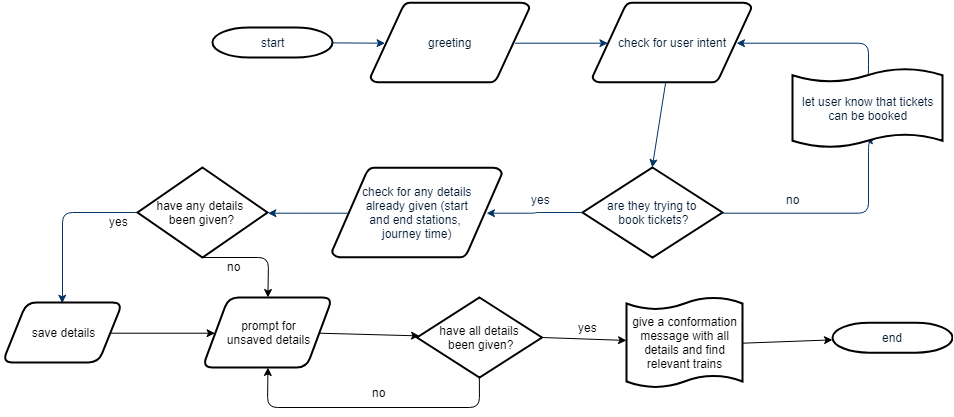
\includegraphics[scale=0.4]{img.png}
        \caption{A flowchart for a simple ticket booking conversation.}
    \end{figure}
    
    \section*{Task 2: An Intelligent Delay Predictor}
    
    The second task involves using historical rail data to predict future delay times, and to collect our historical data, we have used Natoinal Rail's 'Historical Service Performance' API. This has allowed us to create a .csv with roughly 200,000 delays on. Unfortunately, we have only been able to collect delays from one train line (Norwich-London). This is because the API imposes a 5000 request per hour limit. The large number of train routes in Britain means that to collect enough data to make a delay prediction model of the whole country would take far too long for this project. It was decided that data should be collected on just the London Liverpool Street to Norwich route, over the past 2 years. George and Anurag have created a script that pulled the data. \\
    
    Once we have our data, we must take an intelligent approach to predicting future delays. Owen has taken the responsibility of converting the locations and severity of the historical delays into a vector space, so that a modified version of the KNN algorithm can be performed on them. This modified version will classify based on Dempster-Shafer theory \citep{Denoeux95}. This will allow us to predict the delay of any journey, based on past delays.
    
    \section*{Task 3: Contingency Planning}
    
    The final task of this coursework asks our bot to be able to provide guidance and relevant documentation to any staff member dealing with contingencies. Our group has been allocated the contingency "Dealing with Resource Shortages" and for this, Greater Anglia's "Contingency Plan for Service Disruption" document is being used. To complete this task, a knowledge base must be built that can relate any queries to our document. For this, first the document must be broken down into a set of rules. Then, using the PyKnow package, these rules will be able to be interpreted, and our chatbot will know which actions to reccomend.
    
    \section*{Additional Functionality}
    In addition to the functionality outlined above, a database will be implemented to save the details of user's conversations, for example where the user is travelling from and to. This will allow the chatbot to give the user accurate information without the user having to resubmit data to the chatbot.
    
    MongoDB will be used as the database management system (DBMS) as it is widely used and works well with Python. MongoDB is a NoSQL document DBMS that stores data in "flexible, JSON-like documents"\citep{mongodb_2017}. Because of this it makes it very easy to interact with the data using standard data structures like dictionaries.
    
    \section*{Conclusion}
    
    To conclude, Group 4 are making good headway in their tasks. The chatbot is already functioning on Facebook Messenger, and the Azure server is running well. The bot is being tested by some external users, and this is helping with the DialogFlow training. The group are doing well with their allocated tasks, and are excited to deliver the finished chatbot.
    
    % AGSM for harvard referencing
    \bibliographystyle{agsm}
    \bibliography{main}
    
\end{document}
